\documentclass[xcolor=pdftext, table]{beamer}
\usepackage{amsmath, amssymb, amsfonts, latexsym, stmaryrd}
%\usepackage[latin1]{inputenc}
\usepackage[T1]{fontenc}
\usepackage[utf8]{inputenc}
\usepackage[english, spanish]{babel}
% Tabla de tres secciones
\usepackage[flushleft]{threeparttable}

% \toprule, \midrule, \bottomrule
\usepackage{booktabs}
% Tablas con ancho establecido por usuario
\usepackage{tabularx}

% Para diagramas de bloques entre otros
\usepackage{smartdiagram}
\usesmartdiagramlibrary{additions}

% Para vinculos a archivos externos
\usepackage{hyperref}

% tikz
\usepackage{tikz}
\usetikzlibrary{arrows.meta, positioning, shadows}

\usefonttheme{professionalfonts}
%\usetheme{Bergen}
%\usetheme{Hannover}
%\usetheme{Boadilla}
%\usetheme{Luebeck}
\usetheme{Warsaw}
%\usetheme{AnnArbor}

\setbeamercovered{transparent}

% Definicion de colores tabla cronograma
\definecolor{colorfa}{rgb}{0.3569,0.608,0.8353}
\definecolor{colorfb}{rgb}{0.4392,0.678,0.2784}
\definecolor{colorfc}{rgb}{1.0000,0.361,0.0000}
\definecolor{colorsem}{rgb}{0.1804,0.455,0.7098}
\definecolor{colorfd}{rgb}{0.9294,0.490,0.1922}
\definecolor{colorfe}{rgb}{0.2667,0.329,0.4157}

% Definicion comandos tabla cronograma
\newcommand{\fa}{\cellcolor{colorfa}}
\newcommand{\fb}{\cellcolor{colorfb}}
\newcommand{\fc}{\cellcolor{colorfc}}
\newcommand{\sem}{\cellcolor{colorsem}}
\newcommand{\fd}{\cellcolor{colorfd}}
\newcommand{\fe}{\cellcolor{colorfe}}
\newcommand{\fg}{\cellcolor{colorfa}}
\newcommand{\fj}{\cellcolor{colorfb}}

% Definicion de tipos de columnas tabla
\newcolumntype{C}[1]{>{\centering}m{#1}}
\newcolumntype{L}[1]{>{\raggedleft}m{#1}}
\newcolumntype{R}[1]{>{\raggedright}m{#1}}

\setbeamertemplate{headline}{%
	\leavevmode%
	\hbox{%
		\begin{beamercolorbox}[wd=\paperwidth,ht=2.5ex,dp=1.125ex]{palette quaternary}%
			\insertsectionhead
		\end{beamercolorbox}%
	}
}

\setbeamertemplate{footline}
{
	\leavevmode%
	\hbox{%
		%\begin{beamercolorbox}[wd=.4\paperwidth,ht=2.25ex,dp=1ex,center]{author in head/foot}%
		%\usebeamerfont{date in head/foot}
		%\insertshortauthor
		%\end{beamercolorbox}%
		%\begin{beamercolorbox}[wd=.6\paperwidth,ht=2.25ex,dp=1ex,center]%
		\begin{beamercolorbox}[wd=0.9\paperwidth,ht=2.25ex,dp=1ex,center]%
			{title in head/foot}%
			\usebeamerfont{title in head/foot}\insertshorttitle\hspace*{3em}
			%\insertframenumber{} / \inserttotalframenumber\hspace*{1ex}
		\end{beamercolorbox}%
		\begin{beamercolorbox}[wd=0.1\paperwidth,ht=2.25ex,dp=1ex,center]%
			{author in head/foot}%		
			\insertframenumber{} / \inserttotalframenumber\hspace*{1ex}
		\end{beamercolorbox}%		
		}%
	\vskip0pt%
}

\setbeamertemplate{note page}[plain]

\begin{document}
	\title{Seminario Trabajo Especial de Grado}
	
	\subtitle{\large DISEÑO DE UN EQUIPO ELECTRÓNICO CONTROLADOR DE
		INTERRUPTORES Y ATENUADORES EMPLEADO EN LA
		MEDICIÓN DE LA FIGURA DE RUIDO EN DISPOSITIVOS DE
		RADIO FRECUENCIA}
		
	\author{{\bf Jose A. Arias B.} \\
		{Tutor: MSc. Pedro Ruiz}\\
		{Prof. Guía: MSc. Alejandro González}}				

		
	\institute{	
		Universidad Central de Venezuela \\
		Facultad de Ingeniería \\
		Escuela de Ingeniería Eléctrica \\
		Departamento de Electrónica, Computación y Control}
	
	\date{Febrero 2018}
	
	%\logo{\includegraphics[height=1.5cm]{Imagenes/pie-der.pdf}}
	
	\frame{\titlepage}
	
	\section{Planteamiento del Problema}
	
% FRAME 1 --------------------------------------------------------------------------------------
	
	\begin{frame}
		\frametitle{Sistema para medición de figura de ruido (SMFR)}	
	
		\begin{figure}		
			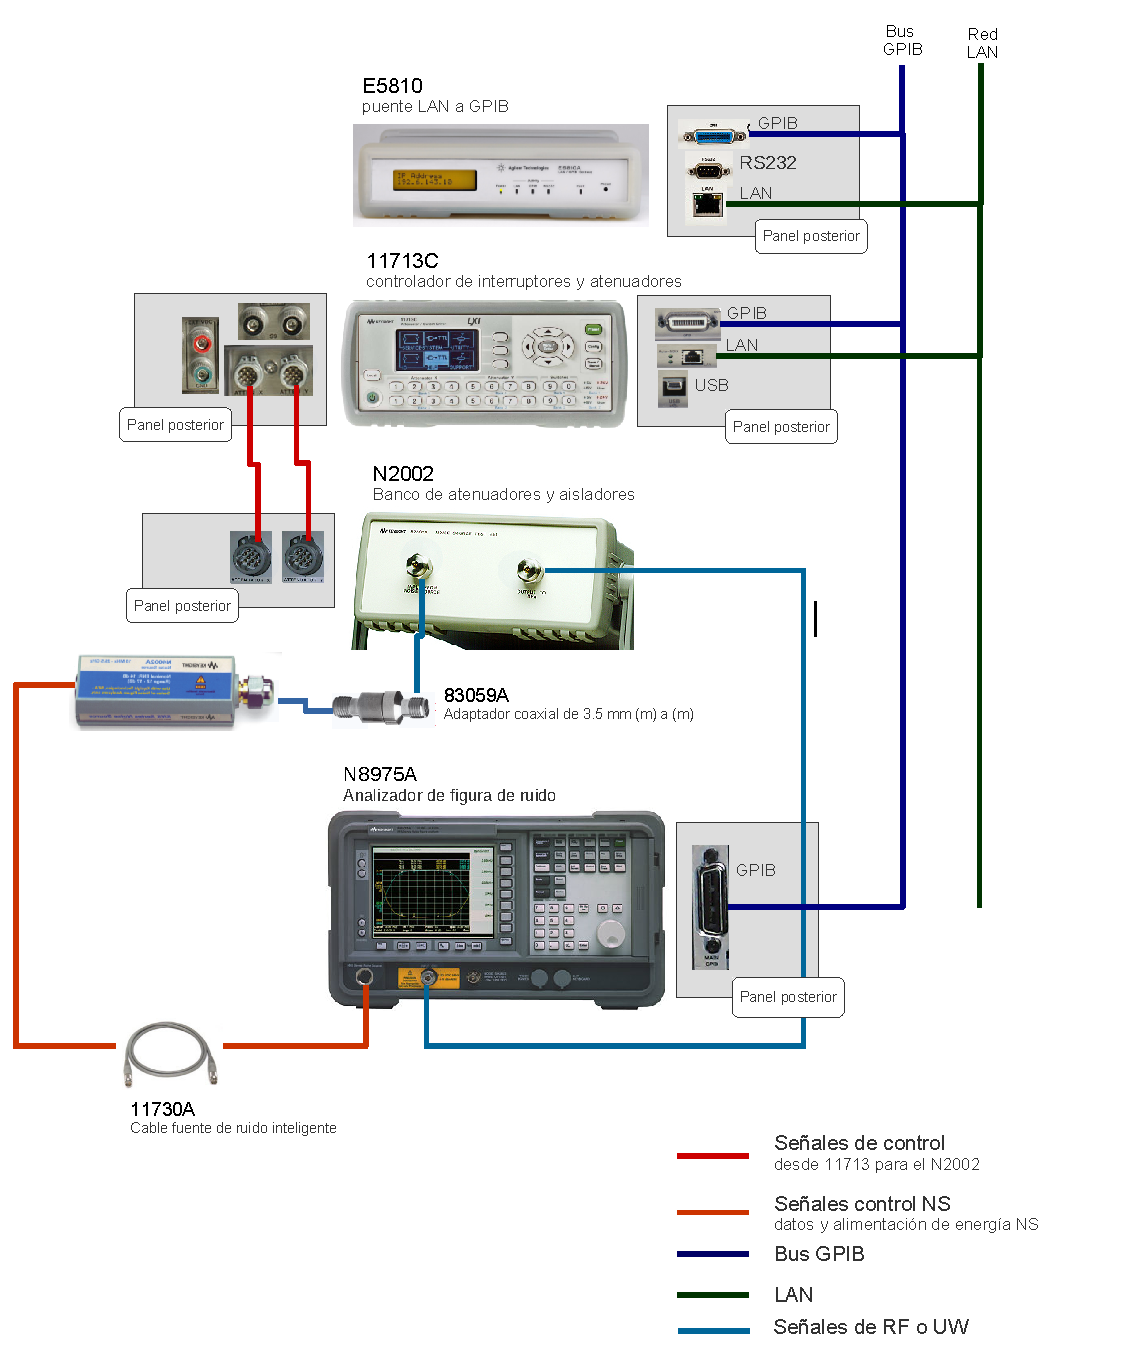
\includegraphics[height=4cm]{Imagenes/SistemaMedicionFiguraRuido.pdf}	
		\end{figure}			

		\begin{table}
			\tiny		
			%\resizebox{12cm}{!}{
			\begin{tabular}{p{2.5cm}p{2.5cm}p{2.5cm}p{2.5cm}}
			%\begin{tabular}{cccc}
				\begin{minipage}{2.5cm}
					\includegraphics[width=2.5cm]{Imagenes/N8975A.pdf}				
				\end{minipage} &	
				\begin{minipage}{2.5cm}
					\includegraphics[width=2.5cm]{Imagenes/N2002A.pdf}
				\end{minipage} &							
				\begin{minipage}{2.5cm}
					\includegraphics[width=2.5cm]{Imagenes/11713A.pdf}
				\end{minipage} &	
				\begin{minipage}{2.5cm}
					\includegraphics[width=2.5cm]{Imagenes/11713B.pdf}
				\end{minipage} \\
													
				{N8975A} &
				{N2002A} &									
				{11713A} &
				{11713C} \\
				
				{Analizador de figura de ruido (NFA)} &
				{Unidad de atenuadores y aisladores} &	
				
				\multicolumn{2}{c}{Controlador electrónico de interruptores y atenuadores} \\
				
			\end{tabular}
			%}	
		\end{table}	
	\end{frame}
	
% FRAME 2 --------------------------------------------------------------------------------------

	\begin{frame}
		\frametitle{Panorama del SMFR}			
	
		\begin{figure}
			\begin{center}
				\includegraphics[width=10cm]{Imagenes/DiagramaBloquesSistema.pdf}
			\end{center}
		\end{figure}	
	
	\end{frame}
	
	\section{Objetivos} 
	
% FRAME 3 --------------------------------------------------------------------------------------
	
	\begin{frame}
		\frametitle{Objetivo general}		
		
		\begin{block}{}
			\centering
			Diseñar un equipo electrónico que permita emular las características funcionales de un controlador electrónico de interruptores y atenuadores.
		\end{block}
		
		\begin{center}			
			\small 
			 El título del proyecto y su objetivo general permanecen sin cambios
		\end{center}
		
	\end{frame}
	
% FRAME 4 --------------------------------------------------------------------------------------	
	
	\begin{frame}
		\frametitle{Objetivos específicos}		

		\begin{small}
			\begin{block}{}		
				\begin{itemize}
					\item Realizar una investigación documental sobre caracterización de dispositivos de radio frecuencia y la medición de figura de ruido sobre éstos.	
											
					\item Recopilar la documentación y software asociado al sistema de medición de figura de ruido (SFMR).	
					
					\item Codificar una librería de software para intercambio de datos entre un PC y el SMFR.
					
					\item Diseñar y codificar el firmware para dispositivo.
					
					\item Diseñar y construir las tarjetas electrónicas PCB para cada uno de los módulos del equipo: expansores de puertos, fuente de alimentación y tarjeta madre. 
					
					\item Desarrollar una aplicación de software para gestión de la medición de figura de ruido con el SMFR.
					
					\item Generar manuales de usuario para el equipo y para la aplicación.	
				\end{itemize}				
			\end{block}
		\end{small}
		
	\end{frame}
	
% FRAME 5 --------------------------------------------------------------------------------------	
	
	\section{Alcance}
	
	\begin{frame}
		\frametitle{Cambios en el alcance}
		
		\begin{columns}
			\begin{column}{6cm}
				\begin{block}{Hardware}		
					\small	
					\begin{itemize}				
						\item Interfaz de comunicaciones a través de USB. \\ 
						{\tiny Class Device Communication, full speed.}
						{\tiny Inicialmente se habían propuesto las interfaces GPIB, USB, LAN.}
		
						\item Señales para comandar la unidad de atenuadores y aisladores (N2002A). \\ 
						{\tiny Formada por 2 grupos de 16 señales cada uno.}
								
						\item El panel frontal consistirá de un teclado matricial. \\ 
						{\tiny Con 16 teclas.} 
						{\tiny Se elimina la pantalla LCD táctil.}
					\end{itemize}
				\end{block}	
			\end{column}
			
			\begin{column}{6cm}
				\begin{figure}
					\begin{center}
						\includegraphics[width=6cm]{Imagenes/DiagramaBloquesSistema.pdf}
					\end{center}
				\end{figure}
			\end{column}			
		\end{columns}
		
	\end{frame}
	
% FRAME 6 --------------------------------------------------------------------------------------
	
	\begin{frame}
		\frametitle{Cambios en el alcance}
		
		\begin{block}{Software} 
			\begin{itemize}			
				\item Soporte, a nivel de librerías de software, para establecer comunicación de datos con los dispositivos del SMFR.
				\item Interfaz de usuario gráfica.
				\item Asistencia al usuario durante el ciclo de medición: configuración, ejecución y generación de reportes.
				\item Generación de reportes con resultados de una medición, en formato de documento portable (pdf).
				\item Instalador para la aplicación.
			\end{itemize}	
		\end{block}
		
		
		\begin{block}{Firmware}
			\begin{itemize}
				\item Soporte a las comunicaciones por medio de las interfaz USB.
				\item Gestión de la interacción del usuario con el panel frontal. 	
			\end{itemize}
		\end{block}
		
	\end{frame}	

	\section{Metodología}
	
% FRAME 7 --------------------------------------------------------------------------------------	
	
	\begin{frame}
		\frametitle{Nuevo cronograma de trabajo}
		\begin{block}{}		
			\begin{threeparttable}[!h]
				\centering
				\arrayrulecolor{gray}
				\setlength{\extrarowheight}{4pt}		
				\resizebox{\textwidth}{!}{						
					\begin{tabular}{|c|l|l|l|l|l|l|l|l|l|l|l|l|l|l|l|}
						\hline
							\begin{tabular}{c}
								{\raggedright \textbf{Semanas}} \\
								\hline
								{\raggedleft \textbf{Tareas}}
							\end{tabular}						
						& 1 & 2 & 3 & 4 & 5 & 6 & 7 & 8 & 9 & 10 & 11 & 12 & 13 & 14 & 15\\
						\hline
						Expansor de puertos Viking & \fa & \fa & \fa & \fa & & & & & & & & & & & \\
						\hline				
						Firmware del dispositivo & & & & & & \fc & \fc & \fc & \fc & & & & & & \\ 
						\hline
						Tarjeta madre & & & & & & & & \fd & \fd & \fd & \fd &  & & & \\
						\hline
						Tarjeta de alimentación DC  &  & \fe & \fe & \fe & \fe & & & & & & & & & & \\
						\hline
						Desarrollo de la aplicación SGMFR  & & & & & & &  & \fg & \fg & \fg & \fg & \fg & \fg & \fg & \fg \\
						\hline
						Libro de TEG & & & & & & & & &  & \fj & \fj & \fj & \fj & \fj & \fj \\
						\hline
					\end{tabular}		
				}
				\begin{tablenotes}
					\item {\tiny Fecha de inicio: octubre de 2017.} 
					\item {\tiny Jornada de 8 horas diarias, lunes a viernes, de 8:00 AM a 12:00 M y de 1:30 PM a 4:30 PM.}
				\end{tablenotes}
			\end{threeparttable}		
		\end{block}			
	\end{frame}
	
% FRAME 8 --------------------------------------------------------------------------------------
	
	\begin{frame}
		\frametitle{Cronograma inicial}
	
		\begin{block}{}
			\begin{threeparttable}[!h]
				\centering
				\arrayrulecolor{gray}
				\setlength{\extrarowheight}{4pt}		
				\resizebox{\textwidth}{!}{
					\begin{tabular}{|c|l|l|l|l|l|l|l|l|l|l|l|l|l|l|l|l|l|l|l|l|l|l|l|l|l|l|l|l|}
						\hline 			
						\textbf{Semanas} & 1 & 2 & 3 & 4 & 5 & 6 & 7 & 8 & 9 & 10 & 11 & 12 & 13 & 14 & 15 & 16 & 17 & 18 & 19 & 20 & 21 & 22 & 23 & 24 & 25 & 26 & 27 & 28 \\
						\hline
						\textbf{Fase 1}
						& \fa & \fa & \fa & \fa & \fa & \fa & & & & & & & & & & & & & & & & & & & & & & \\			
						\hline			
						\textbf{Fase 2} & & & & & & & \fb & \fb & \fb & \fb & \fb & \fb & \fb & \fb & \fb & \fb & \fb & & & & & & & & & & & \\
						\hline
						\textbf{Fase 3} & & & & & & & & & & & & & & & & & & \fc & \fc & \fc & \fc & \fc & & & & & & \\	
						\hline		
						\textbf{Seminario} & & & & & & & & & & & & & & \sem & & & & & & & & & & & & & & \\
						\hline
						\textbf{Fase 4} & & & & & & & & & & & & & & & & & & & & & & & \fd & \fd & \fd & \fd &  & \\
						\hline
						\textbf{Fase 5} & & & & & & & & & & & & & & & & & & & & & & & & & & & \fe & \fe \\
						\hline	
					\end{tabular}
				}
				\begin{tablenotes}
					\item {\tiny Fecha de inicio: 6 de Marzo de 2017.} 
					\item {\tiny Jornada de 8 horas diarias, lunes a viernes, de 8:00 AM a 12:00 M y de 1:30 PM a 4:30 PM.}
				\end{tablenotes}
			\end{threeparttable}		
		
			\begin{itemize}
				\tiny
				\item Fase 1: Preparación y documentación.
				\item Fase 2: Diseño de dispositivo.
				\item Fase 3: Implementación de dispositivo.
				\item Fase 4: Producción de manual de usuario. 
				\item Fase 5: Documentación TEG. 				
			\end{itemize}
		
		\end{block}

	\end{frame}

	\section{Resumen de Tareas}
	
% FRAME 9 --------------------------------------------------------------------------------------
		
		\begin{frame}	
			\frametitle{Tareas realizadas}			
			\framesubtitle{desde el último seminario}
			
			\begin{block}{Hardware}					
				\small
				\begin{itemize}
					\item Diseño y construcción de tarjetas PCB.	\\
					\begin{itemize}						
						\item Tarjeta madre basada en PIC18F4550.
						\item Expansor para puertos Viking.
						\item Expansor de puertos para bus GPIB.
						\item Regulador conmutado de +3.3V.
						\item Regulador conmutado de +5.0V.					
					\end{itemize}
					\item Diseño de tarjetas PCB.
					\begin{itemize}
						\item Panel frontal (teclado).
						\item Fuente conmutada principal 120 VAC a +24.0V.
						\item Tarjeta PCB backplane.
					\end{itemize}
					\item Procura de componentes.
				\end{itemize}	
			\end{block}	
					
		\end{frame}
		
% FRAME 10 --------------------------------------------------------------------------------------		
		
		\begin{frame}
			\frametitle{Tareas realizadas}
			\framesubtitle{desde el último seminario}
			\begin{block}{Software}
				\small
				\begin{itemize}									
					\item Diseño de vistas interfaz de usuario.
					\item Codificación de sus controladores.
					\item Librerías de comunicaciones (ajustes, revisión y pruebas).
					\item Librería para gestión de mediciones de NF.
					\item Pruebas.
				\end{itemize}
			\end{block}			
		\end{frame}
		
% FRAME 11 --------------------------------------------------------------------------------------		

		\begin{frame}
			\frametitle{Tareas realizadas}
			\framesubtitle{desde el último seminario}
			
			\begin{block}{Documentación}
				\begin{itemize}
					\item Investigación sobre diseño y modelado de fuentes conmutadas.
					\item Investigación sobre el bus GPIB.
					\item Investigación sobre la programación del NFA (comandos SCPI).
				 \end{itemize}		
			 \end{block}	 
		
		\end{frame}
		
% FRAME 12 --------------------------------------------------------------------------------------		

	\begin{frame} 
		\frametitle{Tareas por completar}
		
		\small
		
		Software		
		\begin{itemize}
			\item  Integración de módulos software {\tiny (interfaz de usuario, librerías gestión de medición y de comunicaciones).}
		\end{itemize}
		
		Hardware		
		\begin{itemize}
			\item Ensamblaje de PCBs {\tiny (tarjeta madre, expansores de puertos y reguladores conmutados).}
			\item Fabricación y ensamblaje de PCBs {\tiny (panel frontal, fuente de alimentación principal y backplane).}
			\item Ensamblaje e integración del dispositivo con aplicación de software.
			\item Manufactura de carcasa.
		\end{itemize}
		
		Firmware
		\begin{itemize}
			\item Gestión de comunicaciones en el bus USB.
			\item Gestión de interfaz de usuario.
			\item Interprete de comandos SCPI.
			\item Control de expansores de puertos {\tiny (gestión de buses I2C y SPI).}
		\end{itemize}
		
	\end{frame}
	
\end{document}